\pagestyle{fancy}
\section{Introducción}

AironTools es una empresa mexicana con más de una década de experiencia en la producción y comercialización de herramientas industriales. A lo largo de su trayectoria ha consolidado una base de clientes recurrentes en el sector metalmecánico y de servicios técnicos. Sin embargo, actualmente enfrenta importantes desafíos operativos derivados del uso de procesos manuales y herramientas no integradas para la gestión interna y la atención a clientes.

La gestión de servicios técnicos, inventario, comunicación interna y control de información se realiza mediante hojas de cálculo y formatos físicos, lo que ha derivado en dificultades para la trazabilidad de los servicios, errores en el registro de información, pérdida de datos importantes para la toma de decisiones, y una experiencia limitada para el cliente, al no contar con un sistema que le permita dar seguimiento a sus solicitudes de manera eficiente.

Estas deficiencias afectan directamente la eficiencia operativa, la competitividad y la capacidad de crecimiento de AironTools frente a otras empresas del sector que ya operan con sistemas digitales robustos e interconectados. En este contexto, se propone el diseño e implementación de un sistema de gestión empresarial que permita digitalizar y automatizar los procesos clave de la organización.

El objetivo del proyecto es desarrollar una plataforma integral que centralice la información, mejore la trazabilidad de los servicios ofrecidos, optimice el control de inventario y facilite la comunicación entre las distintas áreas operativas. Este sistema estará alineado con los flujos de trabajo actuales de la empresa, y se construirá bajo una arquitectura escalable que garantice su adaptabilidad y crecimiento a futuro.

Como beneficio, se espera una mejora sustancial en los tiempos de respuesta, una administración más eficiente de los recursos, una atención al cliente más ágil y profesional, y un fortalecimiento de la capacidad competitiva de AironTools en el mercado de herramientas industriales. El presente proyecto se enmarca dentro de la modalidad de experiencia profesional, y responde a una necesidad real detectada en la operación de la empresa.

\section{Justificación}

La propuesta de este proyecto surge de una necesidad concreta identificada en la operación diaria de la empresa AironTools. En la actualidad, la falta de un sistema de gestión empresarial digitalizado ha derivado en múltiples dificultades operativas, entre las que destacan una atención deficiente al cliente, escasa trazabilidad de los servicios técnicos, desorganización en el control de inventario y una gestión interna basada en registros manuales. Esta situación ha limitado significativamente la capacidad de la empresa para escalar sus operaciones y mantenerse competitiva frente a organizaciones del mismo sector que ya han implementado soluciones tecnológicas robustas.

Los registros actuales de clientes, servicios, inventario y empleados se realizan mediante formatos físicos o archivos aislados, lo cual genera errores frecuentes, pérdida de información, duplicidad de datos y demoras en la atención. Estas deficiencias impactan de manera directa en la eficiencia del personal, en la capacidad de respuesta y en la imagen profesional que la empresa proyecta a sus clientes.

Frente a este panorama, la implementación de un sistema de gestión empresarial integral representa una solución estratégica. Este sistema permitirá centralizar en una sola plataforma la información relacionada con empleados, clientes, servicios y productos, lo que facilitará la trazabilidad del flujo de trabajo desde la solicitud de un servicio hasta la entrega final. Además, la automatización de notificaciones y la digitalización de los procesos permitirán establecer una comunicación más eficiente con los clientes, otorgándoles información puntual y transparente sobre el avance de sus solicitudes.

Otra ventaja clave de esta solución es la optimización del control de inventario. A través de funciones como alertas de stock, reportes automáticos y seguimiento de movimientos, será posible reducir errores, evitar faltantes críticos y anticipar necesidades operativas. A su vez, los reportes generados por el sistema facilitarán la toma de decisiones basadas en datos reales y actualizados, incrementando la capacidad de análisis y planificación de la empresa.

En conjunto, esta propuesta tecnológica contribuirá a mejorar la productividad interna, profesionalizar la operación diaria y elevar la calidad del servicio ofrecido a los clientes. También permitirá documentar formalmente los procesos internos, asegurando su replicabilidad y continuidad. La digitalización de estas funciones no solo responde a una necesidad interna urgente, sino que posiciona a AironTools como una empresa moderna, eficiente y con visión de crecimiento sostenible en un mercado altamente competitivo.

\section{Objetivos}

\subsection{Objetivo General}
Diseñar e implementar un sistema de gestión empresarial digital para AironTools, mediante la automatización y centralización de los procesos internos de atención al cliente, servicios técnicos, control de inventario y comunicación organizacional, con el fin de mejorar la eficiencia operativa, la trazabilidad de los servicios y la calidad del servicio ofrecido.

\subsection{Objetivos Específicos}

\begin{itemize}
	\item Desarrollar un módulo de gestión de usuarios que permita registrar, organizar y asignar roles diferenciados al personal de AironTools según sus funciones operativas.

	\item Implementar un módulo de gestión de clientes que facilite el registro, seguimiento de historial, contacto y servicios solicitados, mejorando la comunicación con el cliente.

	\item Diseñar e implementar un flujo automatizado de servicios técnicos, desde el ingreso del equipo hasta la entrega final, integrando notificaciones en cada etapa.

	\item Desarrollar un módulo de control de inventario que registre entradas, salidas, movimientos de productos y alertas por niveles críticos de stock.
\end{itemize}

\section{Trabajos Relacionados}

A continuación se presentan algunos proyectos y estudios relevantes que han servido como referencia para el desarrollo de esta propuesta, ya sea por su similitud en el enfoque tecnológico, el contexto empresarial o las soluciones planteadas.

\subsection{Digitalización de procesos en empresas manufactureras \cite{Garcia07}}

Este proyecto terminal expone una solución enfocada en la optimización de procesos dentro de empresas manufactureras mediante sistemas digitales. El autor plantea la necesidad de transformar procesos manuales en digitales para aumentar la eficiencia, mejorar el control interno y facilitar el crecimiento. Su propuesta destaca la importancia de integrar herramientas tecnológicas en contextos industriales similares al de AironTools.

\subsection{Automatización en servicios técnicos con enfoque operativo \cite{Nin1992}}

El estudio analiza la implementación de sistemas de automatización en empresas que ofrecen servicios técnicos especializados. Plantea la necesidad de digitalizar el ciclo completo de servicio para reducir errores, mejorar la trazabilidad y elevar la satisfacción del cliente. Es una referencia clave por su enfoque operativo y estructura del flujo técnico.

\subsection{Transformación digital en PyMEs industriales \cite{Rodeiro2012}}

Este artículo explora cómo las pequeñas y medianas empresas del sector industrial pueden abordar la transformación digital para mejorar su competitividad. Estudia los principales factores que afectan la adopción tecnológica y ofrece estrategias de implementación con bajo costo y alto impacto. AironTools comparte características con este tipo de organizaciones.

\subsection{Sistemas de gestión de inventario en el sector de herramientas \cite{Flores2015}}

Este trabajo de maestría describe la implementación de un sistema de gestión de inventario en una empresa cooperativa del sector ferretero. Se destacan los beneficios de tener visibilidad en tiempo real del stock, con reducción en pérdidas y mejora en el control operativo. La propuesta para AironTools se inspira en este enfoque específico de productos físicos.

\subsection{Importancia de la comunicación interna digitalizada \cite{Reyes2012}}

El estudio plantea que una comunicación interna efectiva dentro de una organización mejora la productividad y la coordinación entre departamentos. Propone el uso de plataformas digitales como solución a los problemas de fragmentación en empresas de tamaño medio. Este principio será implementado mediante un módulo de mensajería y notificaciones en el sistema para AironTools.

\subsection{Mejora de la experiencia del cliente mediante sistemas integrados \cite{Patino2019}}

Esta investigación de grado evalúa cómo la planificación estratégica y la integración de sistemas digitales influyen en la percepción del cliente y la fidelización. A través de un caso práctico en una empresa de servicios, se identifican elementos clave para mejorar la comunicación y seguimiento. AironTools podría beneficiarse de aplicar estos principios en su flujo de servicios técnicos.

\begin{longtable}{|p{0.24\textwidth}|p{0.23\textwidth}|p{0.23\textwidth}|p{0.23\textwidth}|}
	\hline
	\textbf{Referencia}                                               & \textbf{Ventajas} & \textbf{Desventajas} & \textbf{Similitudes con el Proyecto} \\
	\hline
	\endfirsthead

	\hline
	\textbf{Referencia}                                               & \textbf{Ventajas} & \textbf{Desventajas} & \textbf{Similitudes con el Proyecto} \\
	\hline
	\endhead

	\hline
	\cite{Garcia07}                                                   &
	\begin{itemize}
		\item Alineado al sector industrial.
		\item Uso de herramientas digitales para procesos internos.
		\item Análisis de eficiencia operativa.
	\end{itemize}       &
	\begin{itemize}
		\item Enfoque general, sin especialización en servicios técnicos.
	\end{itemize} &
	\begin{itemize}
		\item Proceso de digitalización industrial.
		\item Mejora del control interno.
	\end{itemize}                                                                                                          \\
	\hline

	\cite{Nin1992}                                                    &
	\begin{itemize}
		\item Automatización completa del flujo técnico.
		\item Análisis detallado de trazabilidad.
	\end{itemize}                  &
	\begin{itemize}
		\item Tecnología desactualizada.
		\item Escaso enfoque en clientes.
	\end{itemize}                                 &
	\begin{itemize}
		\item Flujo de servicio técnico automatizado.
		\item Seguimiento de procesos.
	\end{itemize}                                                                                                        \\
	\hline

	\cite{Rodeiro2012}                                                &
	\begin{itemize}
		\item Contexto PyME relevante.
		\item Estrategias de adopción tecnológica.
	\end{itemize}                        &
	\begin{itemize}
		\item Poca aplicación práctica directa.
	\end{itemize}                           &
	\begin{itemize}
		\item Enfoque en transformación digital en PyMEs.
	\end{itemize}                                                                                                    \\
	\hline

	\cite{Flores2015}                                                 &
	\begin{itemize}
		\item Enfoque específico en herramientas.
		\item Control detallado del stock.
	\end{itemize}                         &
	\begin{itemize}
		\item Alcance limitado a inventario.
	\end{itemize}                              &
	\begin{itemize}
		\item Gestión de inventario.
		\item Productos industriales físicos.
	\end{itemize}                                                                                                                \\
	\hline

	\cite{Reyes2012}                                                  &
	\begin{itemize}
		\item Mejora de comunicación organizacional.
		\item Énfasis en eficiencia de procesos.
	\end{itemize}                      &
	\begin{itemize}
		\item Sin implementación tecnológica clara.
	\end{itemize}                       &
	\begin{itemize}
		\item Mejora de la comunicación interna en la empresa.
	\end{itemize}                                                                                               \\
	\hline

	\cite{Patino2019}                                                 &
	\begin{itemize}
		\item Orientación al cliente.
		\item Medición de la experiencia del usuario.
	\end{itemize}                     &
	\begin{itemize}
		\item Contexto diferente (empresa propia).
	\end{itemize}                        &
	\begin{itemize}
		\item Satisfacción del cliente y seguimiento del servicio.
	\end{itemize}                                                                                           \\
	\hline
	\caption{Comparación de trabajos relacionados con la propuesta de sistema de gestión empresarial para AironTools.}
	\label{tabla:trabajosRelacionados}
\end{longtable}

\section{Descripción Técnica}

El sistema de gestión empresarial propuesto para AironTools está diseñado como una aplicación web moderna que permite automatizar procesos clave como la atención al cliente, la gestión de servicios técnicos, el control de inventario y la comunicación interna. Se desarrollará utilizando tecnologías actuales que aseguran escalabilidad, seguridad y mantenimiento eficiente.

\subsection{Arquitectura del Sistema}

Se utilizará una arquitectura basada en microservicios, lo cual permitirá escalar módulos de forma independiente, mejorar la tolerancia a fallos y facilitar la implementación modular. Cada servicio podrá operar de forma autónoma y comunicarse con los demás a través de APIs RESTful seguras.

\subsection{Módulos Principales del Sistema}

\begin{itemize}
	\item \textbf{Módulo de Usuarios y Roles}: Gestiona el acceso al sistema mediante autenticación y autorización. Soporta distintos perfiles (administrador, ventas, técnico, etc.).

	\item \textbf{Módulo de Clientes}: Permite registrar y consultar datos de los clientes, sus servicios activos e historial.

	\item \textbf{Módulo de Servicios Técnicos}: Controla el flujo de atención a herramientas, desde su ingreso hasta la entrega. Incluye diagnósticos, cotizaciones, reparaciones y cierre.

	\item \textbf{Módulo de Inventario}: Administra el stock de herramientas, repuestos y productos, con alertas automáticas y reportes de movimientos.

	\item \textbf{Módulo de Notificaciones}: Informa al cliente sobre el estado de sus servicios mediante correo electrónico y alertas internas. También facilita la comunicación entre empleados.
\end{itemize}

\subsection{Tecnologías Utilizadas}

\textbf{Frontend:}
\begin{itemize}
	\item \textbf{React.js} con \textbf{TypeScript} para una interfaz interactiva y mantenible.
	\item \textbf{HTML5} y \textbf{CSS3} para estructura y estilos.
	\item \textbf{Axios} para comunicación con el backend.
	\item \textbf{Figma} y \textbf{Material UI} para diseño de interfaz (UI/UX).
\end{itemize}

\textbf{Backend:}
\begin{itemize}
	\item \textbf{NestJS} con \textbf{TypeScript}, basado en arquitectura modular.
	\item \textbf{MongoDB} como base de datos no relacional por su flexibilidad.
	\item \textbf{Node.js} como entorno de ejecución.
	\item \textbf{Jest} para pruebas automatizadas.
\end{itemize}

\textbf{Otros componentes:}
\begin{itemize}
	\item \textbf{Docker} para contenedores y despliegue.
	\item \textbf{GitHub Actions} para integración y despliegue continuo (CI/CD).
	\item \textbf{Visual Studio Code} como entorno de desarrollo.
\end{itemize}








\section{Especificación Técnica}

El desarrollo del sistema de gestión empresarial para AironTools se basa en un enfoque modular, escalable y centrado en los procesos críticos de la empresa. El sistema será accesible a través de una aplicación web y podrá ser utilizado por empleados autorizados desde distintos dispositivos.

\subsection{Alcance del Proyecto}

El proyecto incluye el diseño, desarrollo e implementación de los siguientes módulos funcionales:

\begin{itemize}
	\item Registro y gestión de empleados con roles diferenciados.
	\item Registro de clientes y su historial de servicios.
	\item Gestión completa del flujo de servicios técnicos.
	\item Control del inventario de herramientas y productos.
	\item Notificaciones automáticas para empleados y clientes.
	\item Comunicación interna por mensajería o correo empresarial.
	\item Generación de reportes operativos.
\end{itemize}

Cada módulo será desarrollado, probado e integrado de forma progresiva para asegurar una implementación ordenada.

\subsection{Tecnologías y Arquitectura}

El sistema utilizará una arquitectura cliente-servidor basada en microservicios. El frontend será desarrollado en \textbf{React.js} y \textbf{TypeScript}, mientras que el backend será implementado en \textbf{NestJS} sobre \textbf{Node.js}. Para el almacenamiento de datos se usará \textbf{MongoDB}, una base de datos NoSQL flexible y escalable.

El sistema se ejecutará en contenedores mediante \textbf{Docker}, y el flujo de integración y entrega continua será gestionado con \textbf{GitHub Actions}.

\subsection{Criterio de Finalización del Proyecto}

El proyecto se considerará finalizado cuando todos los módulos definidos hayan sido desarrollados, integrados y validados mediante pruebas funcionales. Además, deberá estar documentado correctamente y desplegado en un entorno de pruebas funcional.

\begin{itemize}
	\item Todos los módulos deben cumplir con los casos de uso definidos.
	\item Debe existir documentación técnica y manual de usuario.
	\item El sistema debe estar instalado en un servidor funcional o entorno en la nube.
	\item Se debe realizar una presentación funcional ante la Coordinación.
\end{itemize}

\textbf{Figura \ref{fig:componentes-sistema}} muestra la arquitectura general del sistema, y la \textbf{Figura \ref{fig:casos-uso}} representa los principales casos de uso que deben cumplirse para la validación del proyecto.

\vspace{0.5cm}

%Este texto SÍ debe incluirse para que la propuesta pueda ser aceptada.
Al concluir el proyecto de integración se entregará a la Coordinación de Estudios de Ingeniería en Computación una carpeta digital que incluirá el reporte final del proyecto en un archivo PDF (sin restricciones)\footnote{Debe poder visualizarse sin solicitar contraseña}, el código fuente de la aplicación en un archivo comprimido (sin restricciones)\footnote{Debe poder descomprimirse sin solicitar contraseña}. Además, la sección de apéndices del reporte final contendrá al menos un listado del código fuente desarrollado.

\section{Calendario de Actividades}

El desarrollo del proyecto se llevará a cabo durante el trimestre 2025-Invierno, como parte de la UEA "Proyecto de Integración de Ingeniería en Computación I" (clave 1100113), con un valor de 18 créditos y una duración de 198 horas.

A continuación se presenta el calendario de actividades, distribuido en 10 fases principales, cada una con su respectivo número de horas y entregables.

\begin{longtable}{p{0.05\textwidth} p{0.45\textwidth} p{0.1\textwidth} p{0.30\textwidth}}
	\label{table:calendarioActividades}                                                                                                                                               \\
	\toprule
	\textbf{No.} & \textbf{Actividad}                                                           & \textbf{Horas} & \textbf{Entregable}                                                \\
	\hline
	\endfirsthead

	\hline
	\textbf{No.} & \textbf{Actividad}                                                           & \textbf{Horas} & \textbf{Entregable}                                                \\
	\hline
	\endhead

	\hline
	\caption{Listado de actividades a realizar durante el trimestre 2025-Invierno.}
	\endlastfoot

	1            & Levantamiento de requerimientos y análisis del sistema actual en AironTools. & 20             & Documento de requerimientos                                        \\
	\midrule

	2            & Diseño de arquitectura del sistema y definición de módulos.                  & 20             & Diagramas de arquitectura y diseño técnico                         \\
	\midrule

	3            & Desarrollo del módulo de autenticación y gestión de usuarios.                & 25             & Módulo funcional con control de acceso y roles                     \\
	\midrule

	4            & Desarrollo del módulo de gestión de clientes.                                & 20             & Registro, historial y vista de clientes implementados              \\
	\midrule

	5            & Desarrollo del módulo de servicios técnicos (flujo completo).                & 25             & Módulo de flujo de servicio técnico automatizado                   \\
	\midrule

	6            & Desarrollo del módulo de inventario.                                         & 20             & Registro, movimientos y alertas de inventario                      \\
	\midrule

	7            & Implementación de sistema de notificaciones y comunicación interna.          & 20             & Notificaciones por correo, alertas internas y tareas asignadas     \\
	\midrule

	8            & Pruebas funcionales e integración de los módulos.                            & 20             & Reporte de pruebas, casos de uso validados                         \\
	\midrule

	9            & Despliegue en entorno de pruebas y revisión técnica.                         & 15             & Sistema desplegado en servidor y documentación preliminar          \\
	\midrule

	10           & Documentación técnica y elaboración de manual de usuario.                    & 13             & Manual de usuario, guía de instalación y documentación del sistema \\
	\bottomrule
\end{longtable}

\footnotetext{Las actividades fueron diseñadas para cubrir el desarrollo completo del sistema propuesto durante el trimestre, incluyendo análisis, diseño, codificación, pruebas, despliegue y documentación final.}

\section{Factibilidad Técnica, Operativa y Estimación de Costos}

\subsection{Factibilidad Operativa}

La implementación del sistema de gestión empresarial presenta una alta factibilidad operativa en AironTools por las siguientes razones:

\begin{itemize}
	\item \textbf{Adaptabilidad a procesos existentes:} El sistema se diseñará según las necesidades reales y flujos actuales de la empresa.
	\item \textbf{Capacitación gradual del personal:} Se planea una estrategia progresiva de formación para cada área.
	\item \textbf{Soporte técnico disponible:} El responsable del proyecto dentro de la empresa garantizará la continuidad técnica.
	\item \textbf{Aprobación de dirección:} El proyecto cuenta con el respaldo directo del jefe de área: \textbf{Mtro. Víctor Benjamín Aguilar Orocio}.
\end{itemize}

\subsection{Factibilidad Técnica}

El proyecto es técnicamente viable debido a los siguientes elementos disponibles:

\subsubsection{Recursos de desarrollo y pruebas}
\begin{itemize}
	\item Equipos de cómputo con procesadores Intel i7, 16GB RAM y SSDs.
	\item Acceso a entornos locales y remotos para desarrollo y despliegue.
	\item Conectividad de red estable para pruebas multiusuario.
\end{itemize}

\subsubsection{Herramientas utilizadas}
\begin{itemize}
	\item \textbf{Frontend:} React.js + TypeScript, Figma, Material UI.
	\item \textbf{Backend:} NestJS, Node.js, MongoDB.
	\item \textbf{Control de versiones:} Git y GitHub.
	\item \textbf{Despliegue:} Docker, GitHub Actions.
\end{itemize}

\subsubsection{Conocimientos del desarrollador}
\begin{itemize}
	\item Experiencia en diseño de software empresarial.
	\item Conocimientos avanzados en desarrollo fullstack.
	\item Capacidad para realizar pruebas, documentación y despliegue.
\end{itemize}

\subsection{Estimación de Costos}

La siguiente tabla muestra una estimación aproximada de los costos asociados al desarrollo e implementación del sistema durante el trimestre.

\begin{longtable}{|p{0.5\textwidth}|p{0.2\textwidth}|p{0.2\textwidth}|}
	\hline
	\textbf{Rubro}                              & \textbf{Costo mensual (MXN)} & \textbf{Costo trimestral (MXN)} \\
	\hline
	\endfirsthead

	\hline
	\textbf{Rubro}                              & \textbf{Costo mensual (MXN)} & \textbf{Costo trimestral (MXN)} \\
	\hline
	\endhead

	Infraestructura de servidores y pruebas     & \$3,000                      & \$9,000                         \\
	\hline
	Licencias y servicios en la nube            & \$2,000                      & \$6,000                         \\
	\hline
	Desarrollo de software (frontend y backend) & \$25,000                     & \$75,000                        \\
	\hline
	Diseño UI/UX y prototipos                   & \$10,000                     & \$30,000                        \\
	\hline
	Capacitación y soporte al personal          & \$5,000                      & \$15,000                        \\
	\hline
	Pruebas de calidad y documentación          & \$4,000                      & \$12,000                        \\
	\hline
	\textbf{Total estimado}                     & \textbf{\$49,000}            & \textbf{\$147,000}              \\
	\hline
	\caption{Estimación de costos para el desarrollo del sistema propuesto.}
	\label{tabla:costos}
\end{longtable}

\footnotetext{Los costos fueron estimados con base en referencias de mercado y validación interna con el responsable del área. Incluyen desarrollo, pruebas, capacitación e infraestructura necesaria para el trimestre.}


\begin{figure}[H]
	\centering
	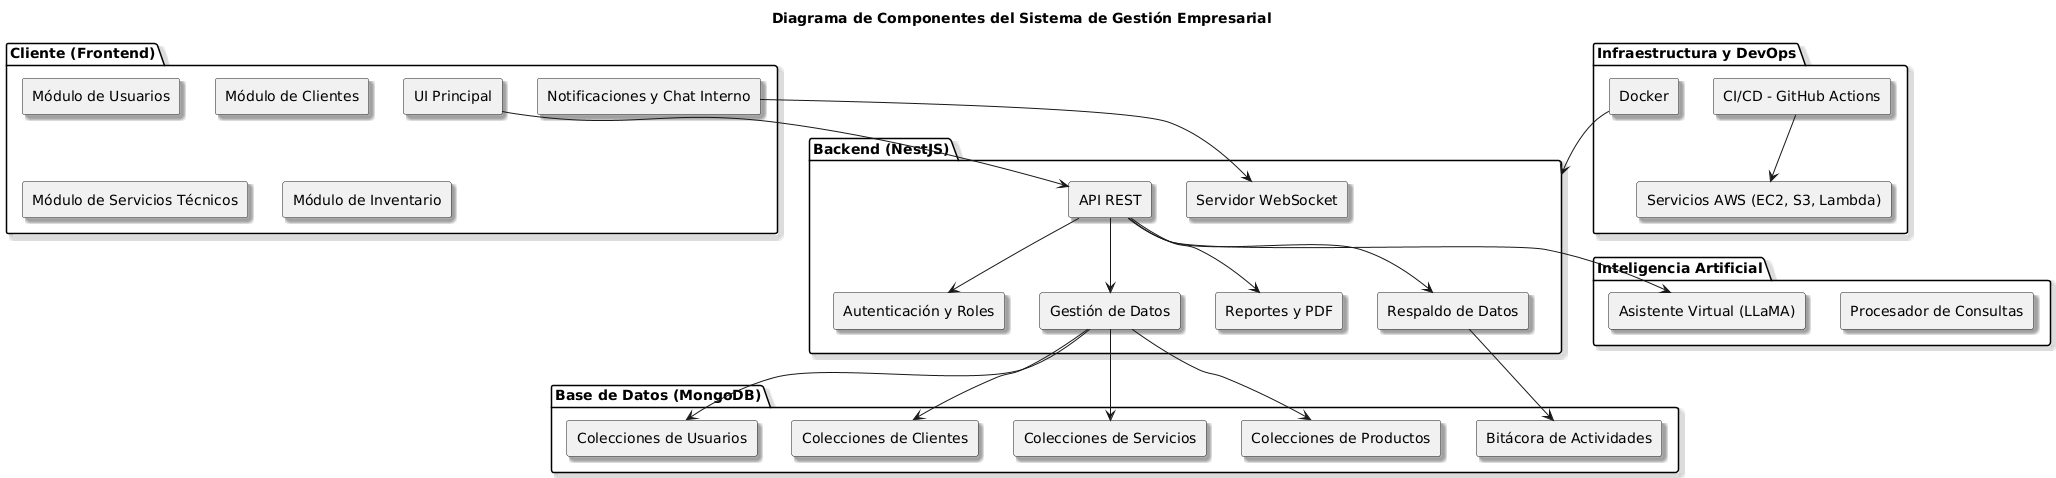
\includegraphics[width=0.8\textwidth]{componentes-sistema.png}
	\caption{Diagrama de Componentes del Sistema}
	\label{fig:componentes-sistema}
\end{figure}


\begin{figure}[H]
	\centering
	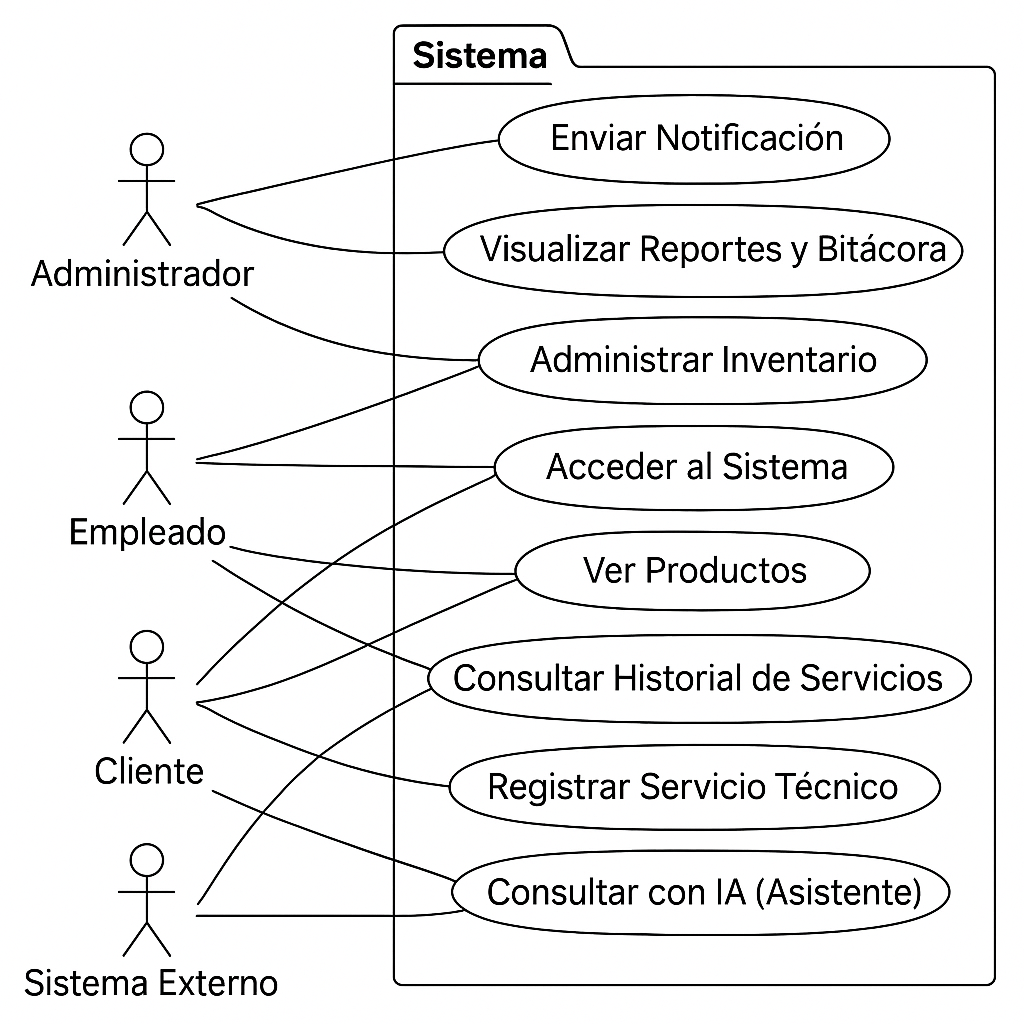
\includegraphics[width=0.8\textwidth]{casos-uso-sistema.png}
	\caption{Diagrama de Casos de Uso del Sistema}
	\label{fig:casos-uso}
\end{figure}


\begin{figure}[H]
	\centering
	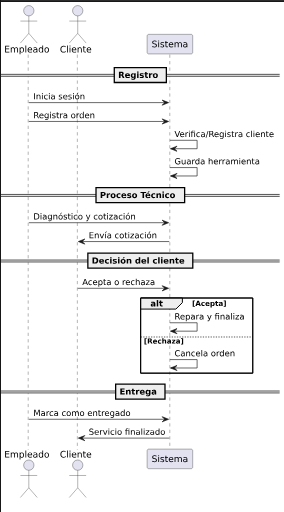
\includegraphics[width=0.8\textwidth]{secuencia-sistema.png}
	\caption{Diagrama de Secuencia del Sistema}
	\label{fig:secuencia-sistema}
\end{figure}


\begin{figure}[H]
	\centering
	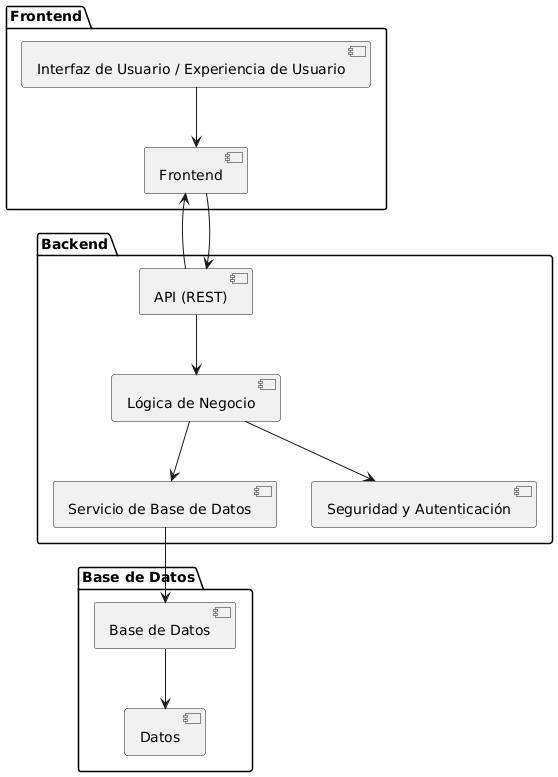
\includegraphics[width=0.8\textwidth]{sistema.png}
	\caption{Vista general del sistema propuesto}
	\label{fig:vista-general}
\end{figure}